\section{Herramientas}
\label{sec:herramientas}
Esta sección incluye un compendio de las herramientas empleadas durante el desarrollo del presente Trabajo Fin de Grado, clasificándolas según su ámbito de aplicación en: herramientas destinadas al producto (\referenciaSeccion{sec:herProducto}), que son aquellas que se emplean para modificar el código fuente o para mantenerlo y divulgarlo en tanto que proyecto \textit{software}; y la herramienta destinada al propio proceso, \textbf{Trello}, que ha sido la empleada para la gestión, organización y jerarquización de las tareas (\referenciaSeccion{sec:herTrello}).

\subsection{Herramientas para el producto}
\label{sec:herProducto}

\subsubsection{Edición de código}
\label{subsec:herIDEs}
Los entornos de desarrollo integrados o IDE (siglas de \textit{Integrated Development Environment}) son aplicaciones informáticas específicamente destinadas a los desarrolladores de proyectos \textit{software}, ya que cuentan con una funcionalidad específicamente destinada al desarrollo con el fin de hacerlo más sencillo.

La composición arquitectónica del proyecto \textit{VSCode4Teaching}, que dispone de tres componentes heterogéneos, conduce intrínsecamente a la necesidad de utilizar varias herramientas especializadas distintas para cada uno de sus componentes.

\textbf{WebStorm}, de JetBrains \cite{WebStorm}, es el entorno de preferencia para ejecutar el presente hito evolutivo que, como se centra en la aplicación web Angular, requiere de un entorno especializado en el desarrollo web. Esta herramienta de JetBrains está específicamente enfocada a la plataforma web y facilita al desarrollador el trabajo con las tecnologías propias de este ámbito, como JavaScript o TypeScript y, en este caso concreto, Node y el \textit{framework} Angular. Es \textit{software} privativo de uso gratuito para aplicaciones educativas y de \textit{software} libre.

La implementación de una extensión para \textbf{Visual Studio Code} hace imperativo el uso del susodicho entorno de desarrollo. Desarrollado por Microsoft y distribuido bajo licencia MIT como \textit{software} libre \cite{VSCode}, es el entorno necesario para la programación de extensiones, ya que brinda herramientas para la fácil ejecución y depuración de las extensiones.

Por otro lado, \textbf{IntelliJ IDEA}, también de JetBrains \cite{IntelliJ}, es una herramienta muy popular para el desarrollo de aplicaciones basadas en la plataforma Java, como es el caso del servidor de \textit{VSCode4Teaching}. Tiene varias extensiones integradas en el propio entorno que facilitan el desarrollo de servicios web y de aplicaciones basadas en Spring. Al igual que WebStorm, es de uso gratuito cuando se destina al ámbito educativo o cuando se emplea para implementar \textit{software} libre.

\subsubsection{Sistema de control de versiones}
\label{subsec:herGit}
Los sistemas de control de versiones son herramientas que ponen a disposición de los programadores partícipes de un proyecto la capacidad para observar y gestionar el cambio producido en el código a lo largo del tiempo, ofreciendo la posibilidad de conservar la historia de un proyecto a través de la sucesión de distintos cambios acontecidos sobre él. Además, estos sistemas incorporan capacidades para que los distintos integrantes de un proyecto puedan trabajar en paralelo, facilitando la posterior incorporación de los distintos cambios acontecidos de diversas formas.

El sistema de control de versiones más extendido en la actualidad es \textbf{git}, que es un ``sistema de control de versiones distribuido, gratuito y de código abierto diseñado para manejar con velocidad y eficacia desde proyectos pequeños hasta muy grandes de forma rápida y eficiente'' \cite{Git}. Distribuido bajo licencia de \textit{software} libre GNU 2.0, git pone a disposición de sus usuarios una herramienta fácil de usar y aprender que se basa en el concepto de ``ramas'' de desarrollo para facilitar que distintos desarrolladores evolucionen el código, posteriormente fusionando sus cambios incorporados en forma de \textit{commits}, que son los pequeños hitos registrados en la historia del proyecto y que hacen referencia a las variaciones realizadas por los desarrolladores en los distintos ficheros de un proyecto.

A pesar de su carácter distribuido, es habitual que los proyectos git tengan como punto de referencia un servidor remoto al que todos los integrantes del proyecto trasladan sus cambios particulares mediante una operación de subida (\textit{push}) y del que todos sincronizan su versión local de la historia a partir de los cambios producidos por otros a través de una operación de actualización (\textit{fetch}) y descarga (\textit{pull}) de los cambios. En el caso de este proyecto, el servidor empleado es GitHub, detallado en la \referenciaSeccion{subsec:tecGitHub}.

\subsubsection{CI/CD: GitHub Actions}
\label{subsec:herCiCd}
CI/CD es una abreviatura formada a partir de tres conceptos: integración continua (del inglés \textit{Continuous Integration}), entrega continua (del inglés \textit{Continuous Delivery}) y despliegue continuo (del inglés \textit{Continuous Deployment}). Forma parte de la filosofía DevOps, que es un ``conjunto de prácticas, herramientas y filosofía cultural que busca automatizar e integrar los procesos que comparten los equipos de desarrollo de \textit{software} y de operaciones'' \cite{DevOps}. A esta filosofía, CI/CD contribuye proponiendo la automatización de los procesos de construcción, validación y despliegue del \textit{software}, promoviendo la necesidad de realizar integraciones por parte del equipo de desarrollo de forma iterativa y ágil, evitando paralizar el ciclo de desarrollo para realizar estas operaciones \cite{CICDRedHat,CICDGitlab}.

\textit{VSCode4Teaching} utiliza \textbf{GitHub Actions}, una herramienta de GitHub que ``facilita la automatización de todos los flujos de trabajo del \textit{software}, [\dots] permitiendo construir, validar y desplegar el código desde GitHub'' \cite{GitHubActions}.

Anteriormente, el proyecto venía utilizando Travis CI como plataforma para ejecutar algunas tareas de la esfera propia de la integración continua, como las ejecución de las baterías de pruebas automáticas del servidor y la extensión y el despliegue de las nuevas versiones del servidor. Este Trabajo Fin de Grado establece en su sexto objetivo (véase el \referenciaCapitulo{cap:objetivos}) la necesidad de mejorar la calidad del proyecto \textit{software} y de, en consonancia, automatizar más tareas relativas a la entrega y despliegue continuos. Como GitHub es la tecnología que se emplea en el proyecto para la conservación y divulgación del código fuente (\referenciaSeccion{subsec:tecGitHub}), se ha decidido cambiar de sistema para CI/CD en favor de GitHub Actions, aprovechando, además, para aumentar su alcance. Esta migración queda materializada a través del requisito no funcional por el que se han implementado los nuevos flujos de trabajo de GitHub Actions, el requisito \texttt{RN-5} (véase la \referenciaSeccion{subsec:rn5}).

\subsection{Organización del proceso \textit{software}: Trello}
\label{sec:herTrello}
Este Trabajo Fin de Grado se ha realizado según un proceso \textit{software} basado en la ejecución de iteraciones reducidas que dan lugar a pequeños incrementos cuya agregación permite alcanzar la nueva evolución pretendida para el proyecto \textit{VSCode4Teaching}. En particular, para la gestión de las tareas, se han tomado como referencia algunas de las técnicas y buenas prácticas que proponen los \textit{frameworks} ágiles Kanban y Scrum, desembocando intrínsecamente en la creación y utilización de un tablero.

Este propósito se ha materializado en la utilización de \textbf{Trello}, que es una ``herramienta visual que permite a los equipos gestionar cualquier tipo de proyecto y flujo de trabajo, así como supervisar tareas'' \cite{Trello}. Esta herramienta permite generar tableros personalizados, pudiendo incluir en cada uno tantas columnas y tarjetas como sea necesario para adecuarlos particularmente a las necesidades de cada proyecto informático.

Trello dota a cada tarjeta dispuesta en un tablero de un sinfín de funcionalidades: además de poder escribir en cada una de ellas un título y una descripción con texto enriquecido, es posible asociarlas ficheros adjuntos, enlaces de interés, listas de tareas anidadas o subyacentes, vínculos a ramas o \textit{commits} de repositorios en GitHub, conexiones con otras tarjetas, clasificación mediante etiquetas de color, comentarios y asignación de autores y fechas de inicio y finalización, entre otras características. La herramienta es intuitiva y visual, lo que facilita la gestión del trabajo realizado, en progreso y pendiente de iniciar de forma rápida y ágil.

En particular, el tablero empleado para la gestión de este proceso toma de Kanban la idea de las tres columnas principales dispuestas: \textit{to do}, que recoge las tareas pendientes de hacer en forma de pila ---es decir, incluye en la parte más alta de la columna la siguiente tarea que será realizada---; \textit{doing}, que alberga la tarea que está siendo ejecutada; y \textit{done}, que agrupa en forma de cola las tareas ya ejecutadas ---esto es, muestra en la parte superior la tarea completada más recientemente---. Por otro lado, se copia de Scrum la idea de disponer de un \textit{product backlog}, que incluye en la primera columna todas las tareas que quedan pendientes de realizar sobre la totalidad del proyecto en forma de pila, extrayendo paulatinamente de él las tareas que se colocan en el \textit{sprint backlog}, que recoge las que se cubrirán en la iteración en curso y que, en este caso, coincide con la columna de tareas pendientes de realización.

La \referenciaFigura{fig:tableroTrello} incluye una instantánea del tablero empleado que permite observar las tarjetas, su colocación en las columnas descritas y la utilización de los elementos visuales de Trello para dar lugar a una visualización colorida e intuitiva que facilita percibir a golpe de vista rasgos básicos del tablero, tales como la cantidad de trabajo pendiente, cuál es la tarea en ejecución o el estado de progreso del proyecto.

Conjugando el modelo de columnas con la visualización incluida en la citada figura, también cabe reseñar la facilidad para la utilización del tablero, ya que todas las tareas fluyen de izquierda a derecha: cuando la tarea en ejecución es finalizada (\textit{doing}), se arrastra a la primera posición de la columna a su derecha (\textit{done}), trasladando la primera de las pendientes de hacer (\textit{to do}) al \textit{doing} para iniciarla. Además, al finalizar cada iteración, se recogen nuevas tarjetas del \textit{product backlog} para fragmentarlas en caso de ser necesario e incluirlas en la columna de tareas pendientes de hacer, ordenándolas por prioridad descendente. Esta sencillez en el uso del método organizativo es crucial, ya que, aunque requiere un esfuerzo inicial mayor para la configuración de la situación inicial del tablero, posteriormente reduce significativamente el esfuerzo y tiempo dedicados a las labores de gestión y planificación de las tareas.

La \referenciaSeccion{sec:metodologia} describe en detalle el proceso \textit{software}, desarrollando con mayor detalle el proceso en su integridad y situando en él la necesidad del tablero de gestión de tareas.

\begin{figure}[ht]
    \centering
    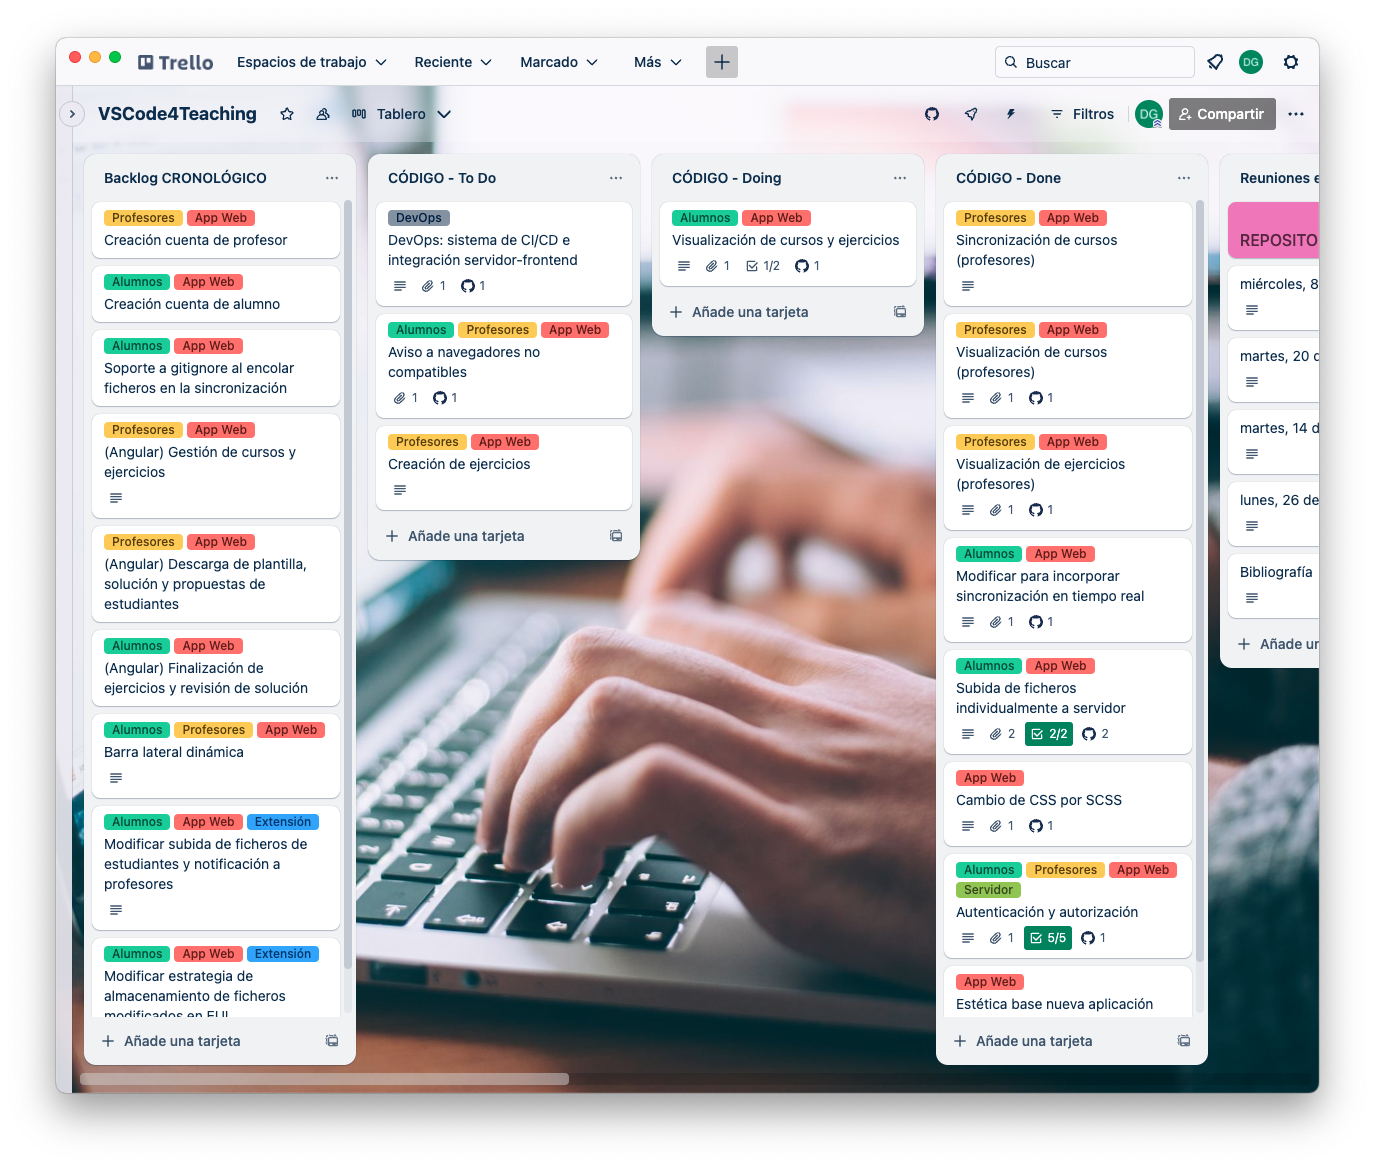
\includegraphics[width=\textwidth]{imagenes/utilizadas/3-2-herramientas/trello.png}
    \caption{Vista del tablero Trello empleado para la gestión del proceso \textit{software}.}
    \label{fig:tableroTrello}
\end{figure}